\usepackage{babel}
\usepackage{microtype}
\usepackage{graphicx}
\usepackage{fancyhdr}
\usepackage{geometry}
\usepackage{abstract}
\usepackage{titlesec}
\usepackage{enumitem}
\usepackage{multirow}
\usepackage{listings}
\usepackage{csquotes}
\usepackage[table]{xcolor}
\usepackage{xurl}
\usepackage{hyperref}
\usepackage{float}
\usepackage{caption}
\usepackage{pdfpages}
\usepackage{nimbusmono}
\usepackage{nimbussans}
\usepackage[T1]{fontenc}
\usepackage{amsmath}
\usepackage{amsfonts}
\usepackage{cleveref}
\usepackage{newfloat}
\usepackage{tikz}
\usepackage{longtable}
\usepackage{array}

%generates filler text
\usepackage{lipsum}
\usepackage[style=ieee,backend=biber,sorting=none]{biblatex}
\addbibresource{bibliography.bib}

\usetikzlibrary{trees}

\setlength{\arrayrulewidth}{0.5mm}
\setlength{\tabcolsep}{12pt}
\renewcommand{\arraystretch}{1.0}

\newcommand{\university}{Politehnica University of Timișoara}
\newcommand{\studyProgram}{Computers and Information Technology}
\newcommand{\academicYear}{2023}
\newcommand{\monthOfPresentation}{June}
\newcommand{\firstName}{Victor Alexandru}
\newcommand{\lastName}{TOPORAN}
\newcommand{\thesisTitle}{Image Processing Demonstration}
% Asist.(SL/Lect./Conf./Prof.)dr.ing.(arh./ec./chim.)
\newcommand{\coordinatorTitle}{Professor Dr. Habil. Eng.}
\newcommand{\coordinatorFirstName}{Mihai V.}
\newcommand{\coordinatorLastName}{MICEA}
\newcommand{\declarationPath}{example_declaration.pdf}

\newcommand{\candidateName}{\firstName{} \MakeUppercase{\lastName}}
\newcommand{\coordinator}{\coordinatorTitle{} \coordinatorFirstName{} \MakeUppercase{\coordinatorLastName}}
\newcommand{\presentationDate}{\monthOfPresentation{} \academicYear{}}

\newcommand*{\blankpage}{
	\null
	\thispagestyle{empty}
	\addtocounter{page}{-1}
	\newpage
}
% set document margins
\geometry{
	left=20mm,
	right=20mm,
	top=25mm,
	bottom=20mm,
	headheight=21mm,
	headsep=4mm
}

% set Nimbus Sans as default font - it is similar to Arial and Helvetica
% Arial is proprietary and it doesn't work with diacritics
\renewcommand*\familydefault{\sfdefault}
\linespread{1.15}
\setlength{\parindent}{1.5cm}

% Link border style
\hypersetup{
	colorlinks   = true,
	urlcolor     = black,
	linkcolor    = black,
	citecolor    = black
}

\lstset{
	numbers=none,
	belowcaptionskip=1\baselineskip,
	breaklines=true,
	frame=l,
	showstringspaces=false,
	basicstyle=\footnotesize\ttfamily,
	% keywordstyle=\bfseries\color{green!40!black},
	% commentstyle=\itshape\color{purple!40!black},
	% identifierstyle=\color{blue},
	% stringstyle=\color{orange}
}

% Disable hyphenation
\pretolerance=10000
\tolerance=2000
\emergencystretch=10pt

%\floatstyle{}
\newfloat{code}{h}{loc}[chapter]

% Set caption names
\floatname{figure}{Figure}
\floatname{table}{Table}
\floatname{code}{Code}

\setlength{\intextsep }{12pt plus 1pt minus 1pt}

% Set citation names
\crefname{code}{Snippet}{Snippet}
\crefname{figure}{Figure}{Figure}
\crefname{table}{Table}{Table}
\crefname{equation}{}{}
\crefname{section}{Section}{Section}
\crefname{chapter}{Chapter}{Capter}
%\renewcommand*{\lstlistlistingname}{Snippet list}

% Make floats centered
\captionsetup{width=0.6\textwidth}

\makeatletter
\g@addto@macro\@floatboxreset\centering
\makeatother




\fancypagestyle{titlepagestyle}{
    \fancyhf{}
    \fancyhead[L]{
        \fontsize{8}{9.6}\selectfont
        \university \\
        \studyProgram \\
    }
    \fancyhead[R]{
        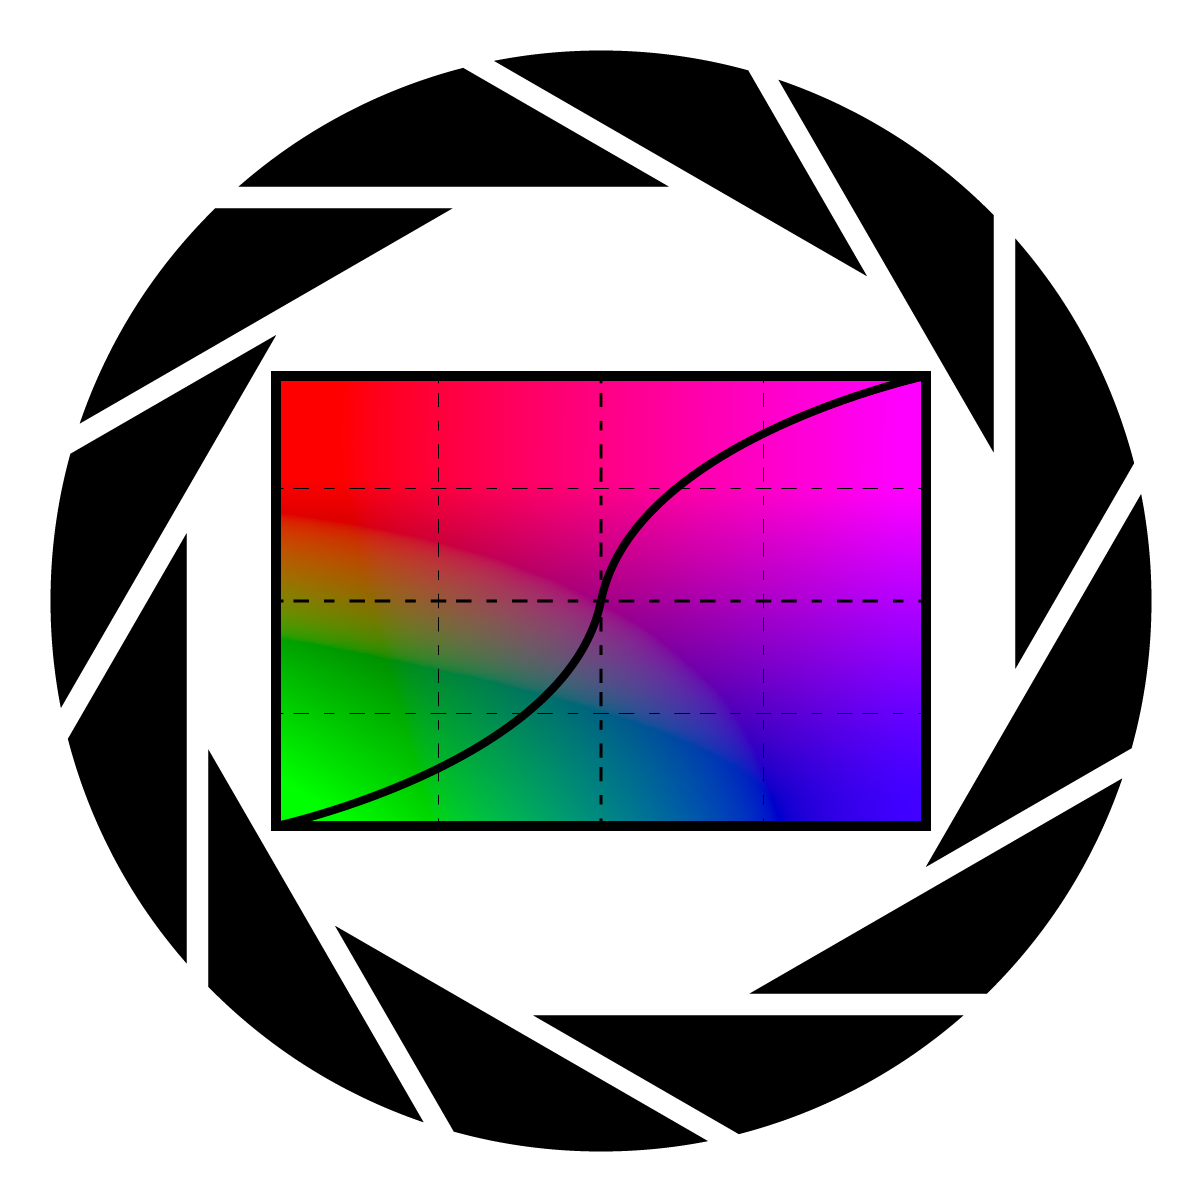
\includegraphics[height=15mm, keepaspectratio]{../src/resources/ISP_Demo_Shutter.png}
        
\includegraphics[height=15mm, keepaspectratio]{images/logo.png}
    }
    \fancyheadoffset[rh]{25mm}
    \renewcommand{\headrulewidth}{0pt}
    \renewcommand\footrulewidth{0pt}
}

\fancypagestyle{abstractpagestyle}{
    \fancyhf{}
    \fancyhead[L]{
    	\fontsize{8}{9.6}\selectfont
		\studyProgram{} \\
        \thesisTitle{} - \thesisSubTitle{} \\
		\candidateName{} \\
        \presentationDate{}
    }
    \fancyhead[R]{
        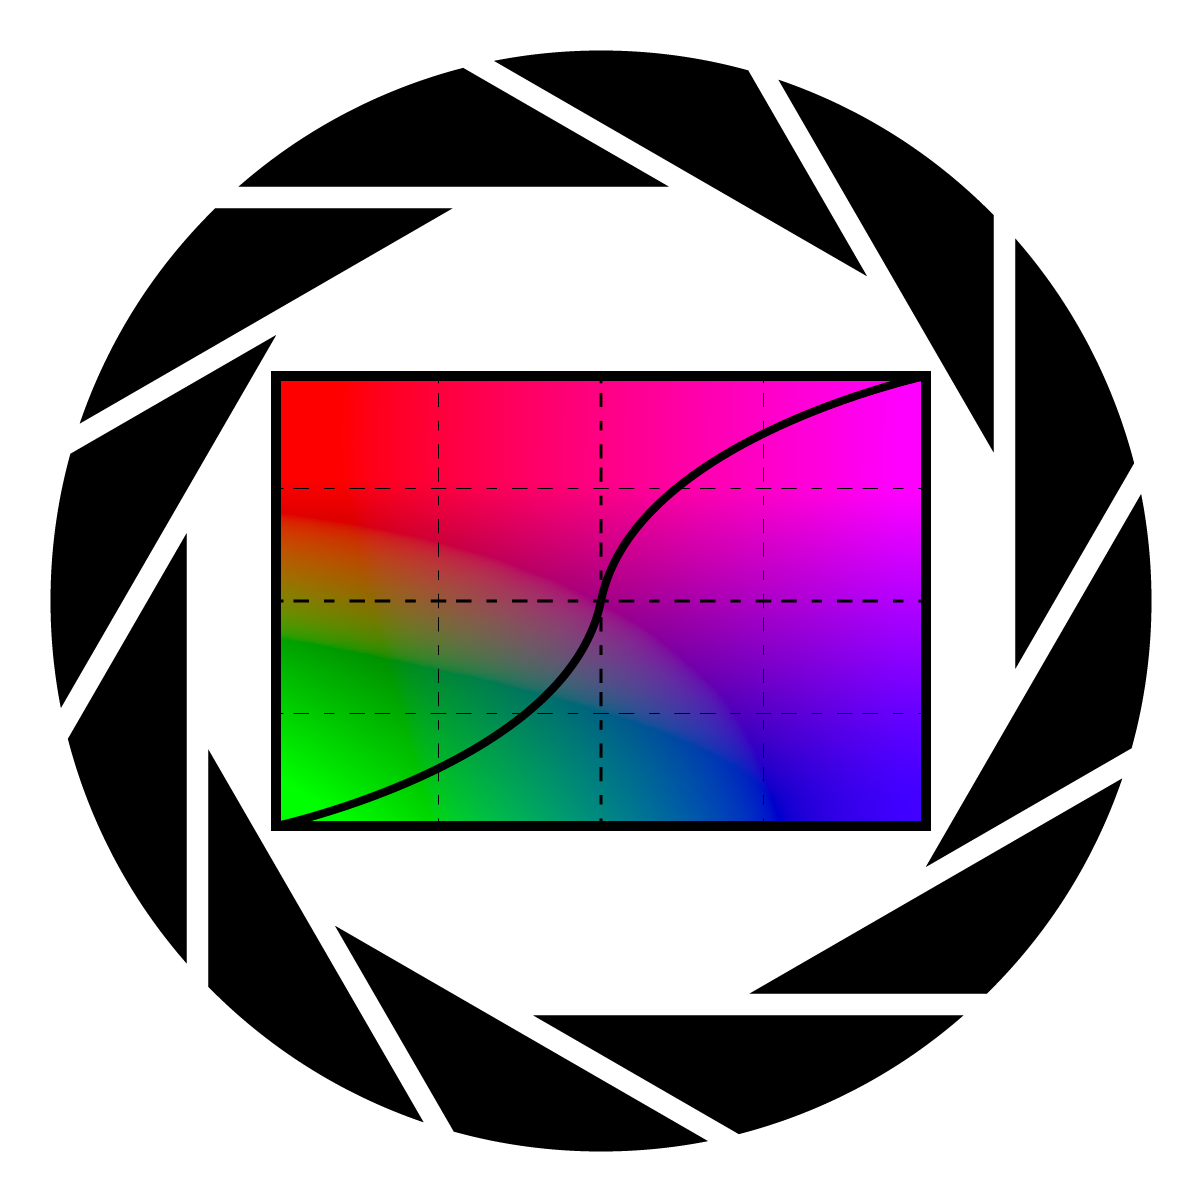
\includegraphics[height=15mm, keepaspectratio]{../src/resources/ISP_Demo_Shutter.png}
        
\includegraphics[height=15mm, keepaspectratio]{images/logo.png}
    }
    \fancyheadoffset[rh]{25mm}
    \renewcommand{\headrulewidth}{0pt}
    \renewcommand\footrulewidth{0pt}
}

\fancypagestyle{pagestyle}{
    \fancyhf{}
    \fancyhead[L]{
        \fontsize{8}{9.6}\selectfont
		\studyProgram{} \\
        \thesisTitle{} - \thesisSubTitle{} \\
		\candidateName{} \\
        \presentationDate{} \\
    }
    \fancyhead[R]{
        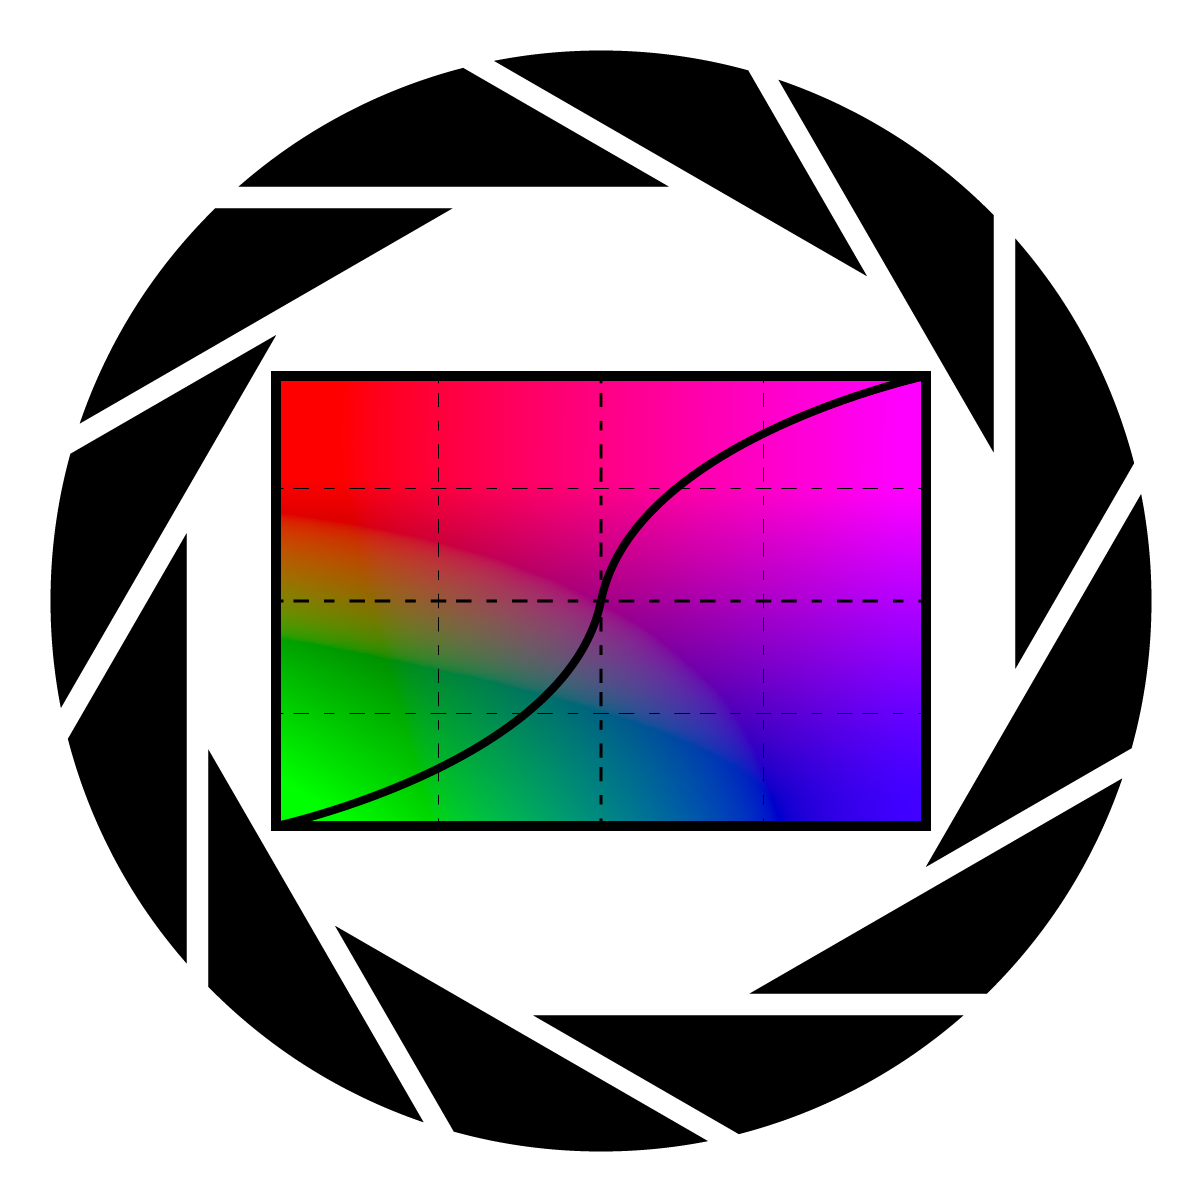
\includegraphics[height=15mm, keepaspectratio]{../src/resources/ISP_Demo_Shutter.png}
        
\includegraphics[height=15mm, keepaspectratio]{images/logo.png}
    }
    \fancyfoot[C]{- {\thepage} -}
    \fancyheadoffset[rh]{25mm}
    \renewcommand{\headrulewidth}{0pt}
    \renewcommand\footrulewidth{0pt}
}

\fancypagestyle{plain}{\pagestyle{pagestyle}}

% set chapter titles format
\titleformat
{\chapter}
[hang]
{\bfseries\fontsize{14pt}{18pt}\selectfont\MakeUppercase} % format
{\thechapter.}
{1em}
{}

\titlespacing
{\chapter}
{0cm}
{0pt}
{24pt}

% set section titles format
\titleformat
{\section}
[hang]
{\bfseries\fontsize{12pt}{16pt}\selectfont\MakeUppercase} % format
{\thesection}
{1.5em}
{}

\titlespacing
{\section}
{0pt}
{12pt}
{12pt}

% set sub section titles format
\titleformat
{\subsection}
[hang]
{\fontsize{12pt}{16pt}\selectfont\MakeUppercase} % format
{\thesubsection}
{2em}
{}

\titlespacing
{\subsection}
{0pt}
{12pt}
{12pt}

\titleformat
{name=\chapter, numberless}
[hang]
{\bfseries\fontsize{14pt}{18pt}\selectfont\MakeUppercase}
{}
{0pt}
{\centering}%

\titlespacing
{name=\chapter, numberless}
{0pt}
{0pt}
{24pt}
%\setlength\cftaftertoctitleskip{8pt}

